\newcommand{\setup}[1]{
%----------------------------------------------------------------------------------------
%	PACKAGES AND OTHER DOCUMENT CONFIGURATIONS
%----------------------------------------------------------------------------------------

    \documentclass[a4paper, 11pt, oneside]{book} % A4 paper size, default 11pt font size and oneside for equal margins

    \usepackage[margin=1in,nomarginpar]{geometry}
    \usepackage[utf8]{inputenc} % Required for inputting international characters
    \usepackage[T1]{fontenc} % Output font encoding for international characters
    \usepackage{fouriernc} % Use the New Century Schoolbook font
    \usepackage{titletoc}% http://ctan.org/pkg/titletoc
    \usepackage{hyperref}
    \usepackage{graphicx}
    \usepackage{lipsum}
    \usepackage{caption}
    \usepackage{float}
    \usepackage{amssymb}
    \usepackage{amsmath}

    \usepackage{xlop}
    \usepackage{tikz}
    \usepackage{xfp}
    \usepackage{soul}
    \usepackage{xifthen}
    \usepackage[]{algorithm2e}
    \sodef\carrystyle{}{0.45em}{0em}{-0.25em}

    \newcommand{\opandbin}[3]{
        \oplogicalbin{##1}{##2}{##3}{$\land$}
    }

    \newcommand{\oporbin}[3]{
        \oplogicalbin{##1}{##2}{##3}{$\lor$}
    }

    \newcommand{\oplogicalbin}[4] {
        \begin{tabular}[t]{rr}
            &\pgfmathbin{##1}\pgfmathresult\\
            ##4&\pgfmathbin{##2}\pgfmathresult\\\hline
            &\pgfmathbin{##3}\pgfmathresult
        \end{tabular}
    }

    \newcommand{\opaddbin}[3]{
        \newcommand{\resultInBaseTen}{\fpeval{##1+##2}}

        \newcount\currentValue
        \newcount\basenumberlength
        \currentValue=\resultInBaseTen
        \basenumberlength=0

        \loop
        \advance \basenumberlength + 1
        \currentValue=\numexpr \currentValue / 2\relax
        \ifnum \currentValue > 1
        \repeat

        \pgfmathsetbasenumberlength{\basenumberlength}
        \begin{tabular}[t]{rr}
            \ifthenelse{\isempty{##3}}%
            {}% if #3 is empty
            {&\pgfcarrybin{##3}\\}% if #3 is not empty
            &\pgfmathbin{##1}\pgfmathresult\\
            +&\pgfmathbin{##2}\pgfmathresult\\\hline
            &\pgfmathbin{\resultInBaseTen}\pgfmathresult
        \end{tabular}
    }

    \newcommand{\pgfcarry}[1]{
        \begin{tiny}
            \expandafter\carrystyle\expandafter{##1}
        \end{tiny}
    }

    \newcommand{\pgfcarrybin}[1] {
        \pgfmathbin{##1}
        \pgfcarry{\pgfmathresult}
    }

    \usepackage{a4wide}
    \usepackage[#1]{babel}
    \usepackage[local,nolabels,exerciseaslist,usesolutionserieslabels]{exsol}
    \renewcommand{\loadSolutions}{
        \immediate\closeout\solutionstream
        \input{\jobname.sol.tex}
        \immediate\openout\solutionstream=\jobname.sol.tex
    }

    \setlength{\exsolexercisetopbottomsep}{0pt plus 0pt minus 1pt}
    \setlength{\exsolexerciseleftmargin}{2em}
    \setlength{\exsolexerciserightmargin}{1em}
    \setlength{\exsolexerciseparindent}{0em}
    \setlength{\exsolexerciselabelsep}{1ex}
    \setlength{\exsolexerciselabelwidth}{30pt}
    \setlength{\exsolexerciseitemindent}{0pt}
    \setlength{\exsolexerciseparsep}{\parskip}

    \usepackage[postpunc={dot},% full stop after description
    nostyles,% don't load default style packages
% load glossaries-extra-stylemods.sty and glossary-tree.sty:
    stylemods={tree}
    ]{glossaries-extra}

    \usepackage[backend=biber,
    style=alphabetic,
    ]{biblatex}

    \usepackage[nottoc]{tocbibind}
    \usepackage{listings}
    \usepackage{xcolor}

    \colorlet{punct}{red!60!black}
    \definecolor{background}{HTML}{EEEEEE}
    \definecolor{delim}{RGB}{20,105,176}
    \colorlet{numb}{magenta!60!black}

    \lstdefinelanguage{json}{
        basicstyle=\normalfont\ttfamily,
        numbers=left,
        numberstyle=\scriptsize,
        stepnumber=1,
        numbersep=8pt,
        showstringspaces=false,
        breaklines=true,
        frame=lines,
        backgroundcolor=\color{background},
        literate=
        *{0}{{{\color{numb}0}}}{1}
        {1}{{{\color{numb}1}}}{1}
        {2}{{{\color{numb}2}}}{1}
        {3}{{{\color{numb}3}}}{1}
        {4}{{{\color{numb}4}}}{1}
        {5}{{{\color{numb}5}}}{1}
        {6}{{{\color{numb}6}}}{1}
        {7}{{{\color{numb}7}}}{1}
        {8}{{{\color{numb}8}}}{1}
        {9}{{{\color{numb}9}}}{1}
        {:}{{{\color{punct}{:}}}}{1}
        {,}{{{\color{punct}{,}}}}{1}
        {\{}{{{\color{delim}{\{}}}}{1}
        {\}}{{{\color{delim}{\}}}}}{1}
        {[}{{{\color{delim}{[}}}}{1}
        {]}{{{\color{delim}{]}}}}{1},
}

% Table of contents with links
\hypersetup{
colorlinks,
citecolor=black,
filecolor=black,
linkcolor=black,
urlcolor=black
}
}
\setup{english}

% glossary
\newglossaryentry{Gloss} {
    name = {Gloss},
    description = {Glossary}
}

\addbibresource{../common/resources/literature.bib}

\usepackage{blindtext} % TODO: Remove

\begin{document}

    %%%%%%%%%%%%%%%%%%%%%%%%%%%%%%%%%%%%%%%%%
% Formal Book Title Page
% LaTeX Template
% Version 2.0 (23/7/17)
%
% This template was downloaded from:
% http://www.LaTeXTemplates.com
%
% Original author:
% Peter Wilson (herries.press@earthlink.net) with modifications by:
% Vel (vel@latextemplates.com)
%
% License:
% CC BY-NC-SA 3.0 (http://creativecommons.org/licenses/by-nc-sa/3.0/)
%
% This template can be used in one of two ways:
%
% 1) Content can be added at the end of this file just before the \end{document}
% to use this title page as the starting point for your document.
%
% 2) Alternatively, if you already have a document which you wish to add this
% title page to, copy everything between the \begin{document} and
% \end{document} and paste it where you would like the title page in your
% document. You will then need to insert the packages and document
% configurations into your document carefully making sure you are not loading
% the same package twice and that there are no clashes.
%
%%%%%%%%%%%%%%%%%%%%%%%%%%%%%%%%%%%%%%%%%

%----------------------------------------------------------------------------------------
%	TITLE PAGE
%----------------------------------------------------------------------------------------

\begin{titlepage} % Suppresses headers and footers on the title page

	\centering % Centre everything on the title page

	\scshape % Use small caps for all text on the title page

	\vspace*{\baselineskip} % White space at the top of the page

	%------------------------------------------------
	%	Title
	%------------------------------------------------

	\rule{\textwidth}{1.6pt}\vspace*{-\baselineskip}\vspace*{2pt} % Thick horizontal rule
	\rule{\textwidth}{0.4pt} % Thin horizontal rule

	\vspace{0.75\baselineskip} % Whitespace above the title

	{\LARGE Die Mathematik neuronaler Netze \\} % Title

	\vspace{0.75\baselineskip} % Whitespace below the title

	\rule{\textwidth}{0.4pt}\vspace*{-\baselineskip}\vspace{3.2pt} % Thin horizontal rule
	\rule{\textwidth}{1.6pt} % Thick horizontal rule

	\vspace{2\baselineskip} % Whitespace after the title block

	%------------------------------------------------
	%	Subtitle
	%------------------------------------------------

	Eine Einführung % Subtitle or further description

	\vspace*{3\baselineskip} % Whitespace under the subtitle

	%------------------------------------------------
	%	Editor(s)
	%------------------------------------------------

	By

	\vspace{0.5\baselineskip} % Whitespace before the editors

	{\scshape\Large Hutzli} % Editor list

	\vspace{0.5\baselineskip} % Whitespace below the editor list

	%\textit{BFH} % Editor affiliation

	\vfill % Whitespace between editor names and publisher logo

	%------------------------------------------------
	%	Publisher
	%------------------------------------------------

	\begin{center}
	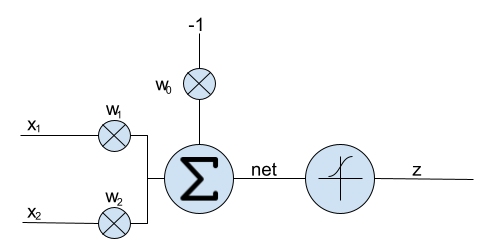
\includegraphics[width=0.8\textwidth]{../common/resources/00_perceptron.png}
	\end{center}

	\vspace{0.3\baselineskip} % Whitespace under the publisher logo

	2021 % Publication year

	{\large No publisher} % Publisher

\end{titlepage}

    \newpage
    \tableofcontents

    \chapter{Chapter 01}
\blindtext~\cite{4767851}

\begin{figure}[h!]
    \begin{center}
        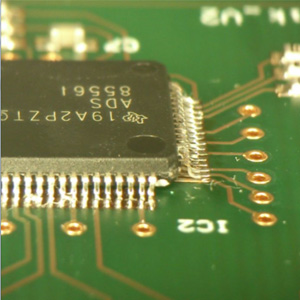
\includegraphics[width=0.2\linewidth]{../common/chapter_01/resources/Elektronik.jpg}
    \end{center}
    \caption{Electronic}
    \label{fig:Electronic}
\end{figure}

\begin{figure}[h!]
    \begin{center}
        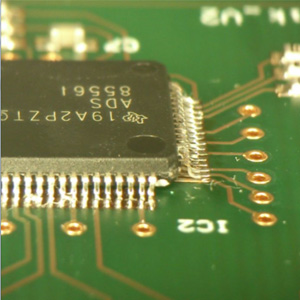
\includegraphics[width=0.2\linewidth]{./chapter_01/resources/Language_specific_resource.jpg}
    \end{center}
    \caption{Language specific}
    \label{fig:Language specific}
\end{figure}

    \newpage
    \listoffigures
    \printbibliography[heading=bibintoc]
    \printunsrtglossary[style={index}]

\end{document}
